\documentclass[11pt]{elegantbook}
\usepackage{graphicx}
%\usepackage{float}
\definecolor{structurecolor}{RGB}{40,58,129}
\linespread{1.6}
\setlength{\footskip}{20pt}
\setlength{\parindent}{0pt}
\newcommand{\argmax}{\operatornamewithlimits{argmax}}
\newcommand{\argmin}{\operatornamewithlimits{argmin}}
\elegantnewtheorem{proof}{Proof}{}{Proof}
\elegantnewtheorem{claim}{Claim}{prostyle}{Claim}
\DeclareMathOperator{\col}{col}
\title{Choice Modeling}
\author{Wenxiao Yang}
\institute{Haas School of Business, University of California Berkeley}
\date{2024}
\setcounter{tocdepth}{2}
\extrainfo{All models are wrong, but some are useful.}

\cover{cover.png}

% modify the color in the middle of titlepage
\definecolor{customcolor}{RGB}{32,178,170}
\colorlet{coverlinecolor}{customcolor}
\usepackage{cprotect}

\addbibresource[location=local]{reference.bib} % bib

\begin{document}
\maketitle

\frontmatter
\tableofcontents

\mainmatter






\chapter{}

\section{Choice Modeling}
\begin{center}
    \fcolorbox{black}{blue!10}{\parbox{.9\linewidth}{\underline{\textbf{Dependent Demand Models}}\\With Choice Models, we can make the demand of offered products to the consumers dependent on the menu of the options.}}
\end{center}
\subsection{Basics}
\begin{enumerate}[$\bullet$]
    \item $N=\{1, \ldots, n\}$ : the potential products,
    \item $S \subseteq N$ : a subset of products that is offered (referred to as assortment).
    \item $\pi_{j}(S)$ : probability that a consumer will purchase product $j$ when $S$ is offered.
    \item $\Pi(S)=\sum_{j \in S} \pi_{j}(S)$ : probability of a sale when $S$ is offered.
    \item $\pi_{0}(S)=1-\Pi(S)$ : probability that the consumer selects outside alternative.
\end{enumerate}
\subsubsection{Assortment Optimization Problem (AOP)}
Let
\begin{enumerate}[$\bullet$]
    \item $p_{j}$ : The price of product $j \in N$.
    \item $z_{j}$ : The unit cost of product $j \in N$.
    \item $p:=\left(p_{1}, p_{2}, \ldots, p_{n}\right)$ : The price vector
    \item $z:=\left(z_{1}, z_{2}, \ldots, z_{n}\right)$ : The unit cost vector.
\end{enumerate}
If we offer $S$, the expected profit from offering subset $S$ is given by:
$$
R(S, z):=\sum_{j \in S}\left(p_{j}-z_{j}\right) \pi_{j}(S)
$$
AOP aims at \underline{finding an assortment $S$} which maximizes $R(S, z)$ :
$$
\mathcal{R}(z):=\max _{S \subseteq N} R(S, z)
$$

\subsubsection{Joint Assortment and Pricing Optimization Problem (JAPOP)}
If the Price is also a Decision Variable, we should solve the following:
$$
\mathcal{R}(z):=\max _{p \geq 0, S\subseteq N} \sum_{j \in S}\left(p_{j}-z_{j}\right) \pi_{j}(S, p)
$$
For many choice models, if $p_{j}=\infty$ then, $\pi_{j}(S, p)=0$. Thus optimizing over prices could implicitly select an assortment.

\subsection{Maximum Utility Models (MUM)}
Suppose a customer has a Full Ordering of the preferences among the products.
\begin{enumerate}[$\bullet$]
    \item Assigns cardinal utilities, say $\{u_i : i \in N\}$, to products and ranks them based on utilities.
    \item The available product with the highest utility is selected with probability $1$.
\end{enumerate}

To introduce randomness into the MUM:
\begin{enumerate}
    \item \textbf{Random Utility Models (RUM):} Add a random noise component to the utilities of the products: $$U_i =u_i +\varepsilon_i,i \in N.$$
    where the $\varepsilon_i$'s are mean zero, possibly dependent random variables.
    \item Assume a distribution of consumer types, each with a certain preference ordering. So, product $i\in S$ is selected by types of consumers for whom $i$ is the highest ranked product in $S$.
\end{enumerate}

\subsection{Basic Attraction Model (BAM)}
\subsubsection{Settings}
\begin{enumerate}[$\bullet$]
    \item In BAM each product has an attraction value $v_j > 0$, capturing attractiveness of product $j$. $v_0>0$ represents the attractiveness of the no-purchase alternative.
    \item The probability of purchasing each item is proportional to the attraction value: $$\pi_j(S)=\frac{v_j}{v_0+\sum_{i\in S}v_i}\quad \forall j\in S$$
\end{enumerate}
Denote, for any $S \subseteq T$:
\begin{enumerate}[$\bullet$]
    \item $\pi_{S}(T):=\sum_{j \in S} \pi_{j}(T)=\frac{\sum_{j \in S}v_j}{v_0+\sum_{i\in T}v_i}=\frac{\sum_{j \in S}v_j}{\sum_{i\in T^+}v_i}$, the probability that a consumer selects a product in $S$ when the set $T$ is offered.
    \item $\pi_{S^{+}}(T):=\pi_{S}(T)+\pi_{0}(T)=\frac{v_0+\sum_{j \in S}v_j}{v_0+\sum_{i\in T}v_i}=\frac{\sum_{j \in S^+}v_j}{\sum_{i\in T^+}v_i}$, including the no-purchase alternative.
\end{enumerate}
\subsubsection{Luce Axioms for BAM}
A discrete choice model satisfies the axioms iff it is of the BAM form:
\begin{enumerate}[$\bullet$]
    \item Axiom 1 :If $\pi_{i}(\{i\}) \in(0,1)$ for all $i \in T$, then for any $Q \subseteq S_{+}$, $S \subseteq T$ :
    $$
    \pi_{Q}(T)=\pi_{Q}(S) \pi_{S_{+}}(T)
    $$
    \begin{proof}
    $\frac{\sum_{i \in Q}v_i}{\sum_{i\in T^+}v_i}=\frac{\sum_{i \in Q}v_i}{\sum_{i\in S^+}v_i}\frac{\sum_{i \in S^+}v_i}{\sum_{i\in T^+}v_i}$
    \end{proof}
    \item Axiom 2: If $v_i=0$ ($\Leftrightarrow$ $\pi_{i}(\{i\})=0$) for some $i \in T$, then for any $S \in T$ such that $i \in S$ :
    $$
    \pi_{S}(T)=\pi_{S \backslash\{i\}}(T \backslash\{i\})
    $$
\end{enumerate}
\subsubsection{Mutinomial Logit Choice Model (MNL): BAM with RUM}
MNL is a special case of BAM, and also has a RUM based justification as well. Specifically:
\begin{enumerate}[$\bullet$]
    \item If $U_{j}=u_{j}+\epsilon_{j}$ for $j \in N_{+}$denotes the random utility of product $j$,
    \item $\epsilon_{j}$ has a Gumbel distribution with zero mean and same scale parameters $\phi$ for all $j$.
\end{enumerate}
- The MNL's probability structure:
$$
\pi_{j}(S)=\frac{e^{\phi u_{j}}}{1+\sum_{k \in S} e^{\phi u_{k}}} \forall j \in S
$$
\underline{\textbf{Gumbel Random Variable:}} Gumbel with location and scale parameters $\nu$ and $\phi$
\begin{enumerate}[$\bullet$]
    \item CDF:
    $
    F(x: \nu, \phi)=\exp (-\exp (-\phi(x-\nu)))
    $
    \item Model: $v$
    \item Median: $v-\ln (\ln 2) / \phi$
    \item Mean: $v+\gamma / \phi$, where $\gamma$ is the Euler constant
    \item Variance: $\pi^{2} / 6 \phi^{2}$
\end{enumerate}

\subsubsection{Mixture of BAMs: Different type consumers}
Denote:
\begin{enumerate}[$\bullet$]
    \item $G$ be the set of consumer types,
    \item $v_{j}^{g}$ : the attraction value of product $j$ for consumer of type $g$.
    \item $\alpha^{g}$ : The probability that a consumer belongs to type $g$.
\end{enumerate}
The Mixture of BAMs suggests the following Probability Structure:
$$
\pi_{j}(S)=\sum_{g \in G} \alpha^{g} \frac{v_{j}^{g}}{v_{0}^{g}+\sum_{i \in S} v_{i}^{g}}
$$
Any RUM-based choice model can be approximated to any degree of accuracy by a mixture of BAM's.

\subsection{Generalized Attraction Model (GAM)}
\subsubsection{Motivation}
The attraction value $v_0$ of the no-purchase option does not depend on the subset of offered products in BAM.

The probability of leaving the store is higher than the one suggested by BAM when eliminating an item.

The BAM ignores the possibility that the consumer may look for the products that are not offered in elsewhere or at a later time.

\subsubsection{Model}
Assume the \textbf{attraction} values $\left\{v_{j}: j \in N\right\}$ for each product $j \in N$

\textbf{Shadow attraction values} $\left\{w_{j}: j \in N\right\}$ with $w_{j} \in\left[0, v_{j}\right]$ for all $j \in N$, which changes the attractiveness of the no-purchase alternative:
$$
v_{0}+\sum_{k \in S^{c}} w_{k}
$$
Note that \underline{in GAM the attractiveness of the no-purchase alternative is dependent on the offered set $S$}.

The probability structure according to the GAM:
$$
\pi_{j}(S)=\frac{v_{j}}{v_{0}+\sum_{k \in S^{c}} w_{k}+\sum_{k \in S} v_{k}}
$$

\subsubsection{Parsimonious GAM: $w_{j}=\theta v_{j}$}
Parsimonious GAM: $w_{j}=\theta v_{j}$ for all $j$ for some $\theta \in[0,1]$.
\begin{enumerate}[$\bullet$]
    \item Independent Demand Model, IDM: If $\theta=1$, the choice probability is independent of $S$ :
    $$
    \pi_{j}(S)=v_{j}
    $$
    where $v_0+\sum_{k\in N}v_k=1$ is normalized.
    \item BAM: $\theta=0$
\end{enumerate}

\subsubsection{Independence of Irrelevant Alternatives (IIA)}
BAM and GAM satisfy the IIA property: adding a new product to an offered subset decrease the purchase probability of all offered products by the same relative amount, i.e., $\forall S\subseteq N$ and $i,j\in S,k\notin S$,
$$\frac{\pi_i(S)}{\pi_i(S\cup\{k\})}=\frac{\pi_j(S)}{\pi_j(S\cup\{k\})}$$

\subsection{Nested Logit Model (to avoid IIA)}
Some products are dependent, we shouldn't count the products in the same nest more than once.

Nested Logit (NL) model, is proposed to avoid IIA. In this model:

The products are organized into nests such that the products in the \textbf{same nest are regarded as closer} substitutes of each other relative to the products in different nests. (Buses in the same nest)

Under the NL model, the selection process of a consumer proceeds in \textbf{two stages}:
\begin{enumerate}[$\bullet$]
    \item First, the consumer selects either \textbf{one of the nests} or decides to leave without making a purchase.
    \item Second, if the consumer selects one of the nests, then the consumer chooses one of the products offered \textbf{in this nest}.
\end{enumerate}
\subsubsection{Notation}
Denote:
\begin{enumerate}[$\bullet$]
    \item $M=\{1, \ldots, m\}:$ the set of nests.
    \item $N$ : set of all items.
    \item $S_{i} \subseteq N$ : the offered set in nest $i$.
    \item $\left(S_{1}, \ldots, S_{m}\right)$ : set of products over all nests.
    \item $v_{i j}$ : attraction value for product $j$ in nest $i$.
    \item $V_{i}\left(S_{i}\right):=\sum_{j \in S_{i}} v_{i j}$.
    \item $\gamma_{i}$ : measure how easily the products in nest $i$ substitute for each other
\end{enumerate}

\subsubsection{Model}
- Given that a consumer has chosen nest $i$, the probability of selecting $j \in S_{i}$ is a BAM:
$$
q_{j \mid i}\left(S_{i}\right):=\frac{v_{i j}}{V_{i}\left(S_{i}\right)}
$$
- \textit{If the items of each nest are more dissimilar, then the probability of choosing nest should increase as it absorbs more kind of consumers.} By this a consumer chooses nest $i$ with probability:
$$
Q_{i}\left(S_{1}, \ldots, S_{m}\right):=\frac{V_{i}\left(S_{i}\right)^{\gamma_{i}}}{v_{i 0}+\sum_{\ell \in M} V_{\ell}\left(S_{\ell}\right)^{\gamma_{\ell}}}
$$
- The selection probability of product $j$ in nest $i$ is given by:
$$
Q_{i}\left(S_{1}, \ldots, S_{m}\right) q_{j \mid i}\left(S_{i}\right):=\frac{V_{i}\left(S_{i}\right)^{\gamma_{i}}}{v_{0}+\sum_{\ell \in M} V_{\ell}\left(S_{\ell}\right)^{\gamma_{\ell}}} \frac{v_{i j}}{V_{i}\left(S_{i}\right)}
$$

\subsubsection{RUM-based justification}
\begin{enumerate}[$\bullet$]
    \item $U_{i j}=u_{i j}+\epsilon_{i j}$
    \item $\epsilon=\left\{\epsilon_{i j}: i \in M, j \in N\right\}$ : generalized extreme value distribution
    $$
    F(x ; \gamma)=\exp \left(-\sum_{i \in M}\left(\sum_{j \in N} \exp \left(-x_{i j} / \gamma_{i}\right)\right)^{\gamma_{i}}\right)
    $$
    \item The marginal distribution of $\epsilon_{i j}$ is Gumbel
    \item For distinct $i, \ell \in M, \epsilon_{i j}$ and $\epsilon_{\ell k}$ are independent
    \item For a given nest $i, \epsilon_{i j}$ and $\epsilon_{i k}$ are positively correlated, and $1-\gamma_{i}$ measures the degree of correlation
\end{enumerate}
The above assumptions lead to NL model with
$$
v_{i j}=\exp \left(u_{i j} / \gamma_{i}\right)
$$




\subsection{Exponomial Choice (EC) Model}
Gumbel distribution makes sense in many cases, particularly those where consumers have limited information regarding a product’s value.

There are many cases, consumers are well-informed about products and prices.
Example: Get information regarding particular cars before purchasing from a dealer.

One might expect the distribution of Willingness to pay (WTP) for a given product across consumers to be negatively skewed.

The utility that a random consumer has for choice $i$ in the EC model is the linear function. $$U_i=u_i-z_i$$
$u_i$ is the ideal utility for choice $i$.

$z_i$ is independent exponential random variables with $\lambda$ rate to capture consumer heterogeneity.

The only difference between EC and MUM is the distribution of $z_i$.

The probability that a consumer prefers choice $i$ is
$$
\begin{aligned}
Q(i) &=\operatorname{Prob}\left\{u_{i}-z_{i} \geq u_{j}-z_{j} \forall j, j \neq i\right\} \\
&=\operatorname{Prob}\left\{z_{j} \geq u_{j}-u_{i}+z_{i} \forall j, j \neq i\right\} \\
&=\int_{0}^{\infty} \prod_{j \neq i}\left[1-F\left(u_{j}-u_{i}+z\right)\right] f(z) \mathrm{d} z
\end{aligned}
$$
where $f(z)=\lambda e^{-\lambda z}$ and $F(z)=1-e^{-\lambda z}$ for $z \geq 0$

\begin{theorem}[Alptekinoğlu and Semple, 2016]
    Out of $m$ choices with utilities $U(i)=u_{i}-z_{i}$, where $u_{1} \leq \cdots \leq u_{m}$ and $z_{i}$ follow independent exponential distributions with rate $\lambda$, the probability that the consumer prefers choice $i \in\{1, \ldots, m\}$, i.e., considers it as utility-maximizing, is
    $$
    Q(i)=\frac{\exp \left[-\lambda \sum_{j=i}^{m}\left(u_{j}-u_{i}\right)\right]}{m-i+1}-\sum_{k=1}^{i-1} \frac{\exp \left[-\lambda \sum_{j=k}^{m}\left(u_{j}-u_{k}\right)\right]}{(m-k)(m-k+1)}
    $$
\end{theorem}
Remark: The parameters of the exponomial model are easy to estimate.

\subsection{Random Consideration Set Model (RCS)}
- An ordering for the preferences of the products:
$$
0 \prec 1 \prec 2 \prec \cdots \prec n
$$
- The consumer forms a consideration set $C(S)$, by independently including each product with probability $\lambda_{i}$.

- For a consumer to purchase product $i$ :

1. Product $\mathbf{i}$ should be in her consideration set,

2. all offered products that are preferred to product $i$ should NOT be in her consideration set.

Thus:
$$
\pi_{i}(S)=\lambda_{i} \prod_{i \prec j, j \in S}\left(1-\lambda_{j}\right) \quad \forall i \in S
$$
- MUM can be recovered when we set $\lambda_{\mathbf{j}}=1, \forall j \in N$.
- Assume consumers pay no attention to the products below the no-purchase alternative and $\lambda_{0}=1$. Then
$$
\pi_{0}(S)=\prod_{j \in S}\left(1-\lambda_{j}\right)
$$
- The RCS model is a \underline{special case of the Markov Chain choice model}.


\subsection{Markov Chain (MC) Choice Model}
First, note that this is an approximation for the underlying choice models.
Thus, the justification of the model is based on the fact that it can approximate other models that are Random Utility Based.

In general: substitution behavior is modeled as a sequence of state transitions of a Markov chain.

In particular:
\begin{enumerate}[(1)]
    \item There is a state for each product including the no-purchase alternative,
    \item A consumer arrives in the state corresponding to his most preferable product,
    \begin{enumerate}[$\bullet$]
        \item If that product is \textbf{available}, she purchases that product and exits.
        \item If that product is \textbf{not available}, she transitions to other product states according to the transition probabilities of the Markov chain.
    \end{enumerate}
\end{enumerate}

\begin{enumerate}[$\bullet$]
    \item Markov chain choice model provides a \underline{good approximation to any random utility discrete choice models} under mild assumptions.
    \item If the choice probabilities used to compute the Markov chain model parameters is generated from an \textbf{underlying GAM}, then the choice probability computed by the Markov chain model coincides with the probability given by the GAM model for all products and all assortments. Thus: \textbf{Exact Approximation}.
    \item Since \textbf{MNL} is a special case of GAM, Markov Chain gives an \textbf{Exact Approximation} of this model as well.
\end{enumerate}

\subsubsection{Notation}
- $\mathcal{N}=\{1,2, \ldots, n\}$ : Universe of products,

- 0: No-Purchase Product,

- $S \subseteq \mathcal{N}$ : offered set,

- $S_{+}:=S \cup\{0\}, \mathcal{N}_{+}=\mathcal{N} \cup\{0\}$,

- $\pi(j, S)$ : the choice probability of item $j \in S_{+}$,

- The set of states: $\mathcal{N}_{+}$,

\subsubsection{How it works}
(1) For any $i \in \mathcal{N}_{+}$, a consumer arrives in state $i$ with probability $\lambda_{i}=\pi(i, \mathcal{N})$.

(2) Selects $i$ if it is available.

(3) o.w. It transitions to another state $j \neq i$, with probability $\rho_{i j}$.

(4) After transitioning to state $j$, the consumer behaves exactly like a consumer whose most preferable product is $j$.

Note that: Substitution arising from a preference list by a Markovian transition model where transitions out of state $i$ do not depend on the previous transitions.

The model is completely specified by:
1 Initial Arrival Probabilities $\lambda_{i}$ for all states $i \in \mathcal{N}_+$,

2 The Transition Probabilities: $\rho_{ij}$, for all $i \in \mathcal{N}$ and $j \in \mathcal{N}_+$.

Note that one of the states is the no-purchase alternative i.e. $0 \in \mathcal{N}_+$.

\subsubsection{Compute Parameters}
Given the choice probabilities for the following $(n+1)$ assortments:
$$
\mathcal{L}=\{\mathcal{N}, \mathcal{N} \backslash\{i\} \mid i=1, \ldots, n\}
$$
Then the parameters are calculated as follows:
$$
\begin{gathered}
\lambda_{i}=\pi(i, \mathcal{N}) \\
\rho_{i j}= \begin{cases}1, & \text { if } i=0, j=0 \\
\frac{\pi(j, \mathcal{N} \backslash\{i\})-\pi(j, \mathcal{N})}{\pi(i, \mathcal{N})} & \text { if } i \in \mathcal{N}, j \in \mathcal{N}_{+}, i \neq j \\
0, & \text { otherwise }\end{cases}
\end{gathered}
$$
The above are pretty intuitive.

- Denote by $\Phi_{j}(S)$ the probability that a consumer considers product $j \notin S$ during the course of her choice process but does not purchase because $j \notin S$.

- By definition, $\Phi_{j}(S)=0$ for all $j \in S$.

- The quantities $\pi_{j}(S)$ for $j \in S$ and $P_{i j}(S)$ for $j \in \bar{S}$, where $\bar{S}=N \backslash S$ are related by the system of equations
$$
\begin{aligned}
&\pi_{j}(S)=\lambda_{j}+\sum_{i \in \bar{S}} \Phi_{i}(S) \rho_{i j} \forall j \in S \\
&\Phi_{j}(S)=\lambda_{j}+\sum_{i \in \bar{S}} \Phi_{i}(S) \rho_{i j} \forall j \in \bar{S}
\end{aligned}
$$

\subsection{Contextual MNL Model}
\begin{definition}[Context Effects]
    Context effects are referred to the changes in the perception about preferability of a given alternative that depend on the presence or absence of other options beside the given alternative. (Note NOT talking about demand.)
\end{definition}
\begin{enumerate}[$\bullet$]
    \item \textbf{The Attraction Effect-Decoy Effect:} An asymmetrically dominated item is the one which is dominated by just
    one of the items of the choice set and not the other.
    \begin{center}\begin{figure}[htbp]
        \centering
        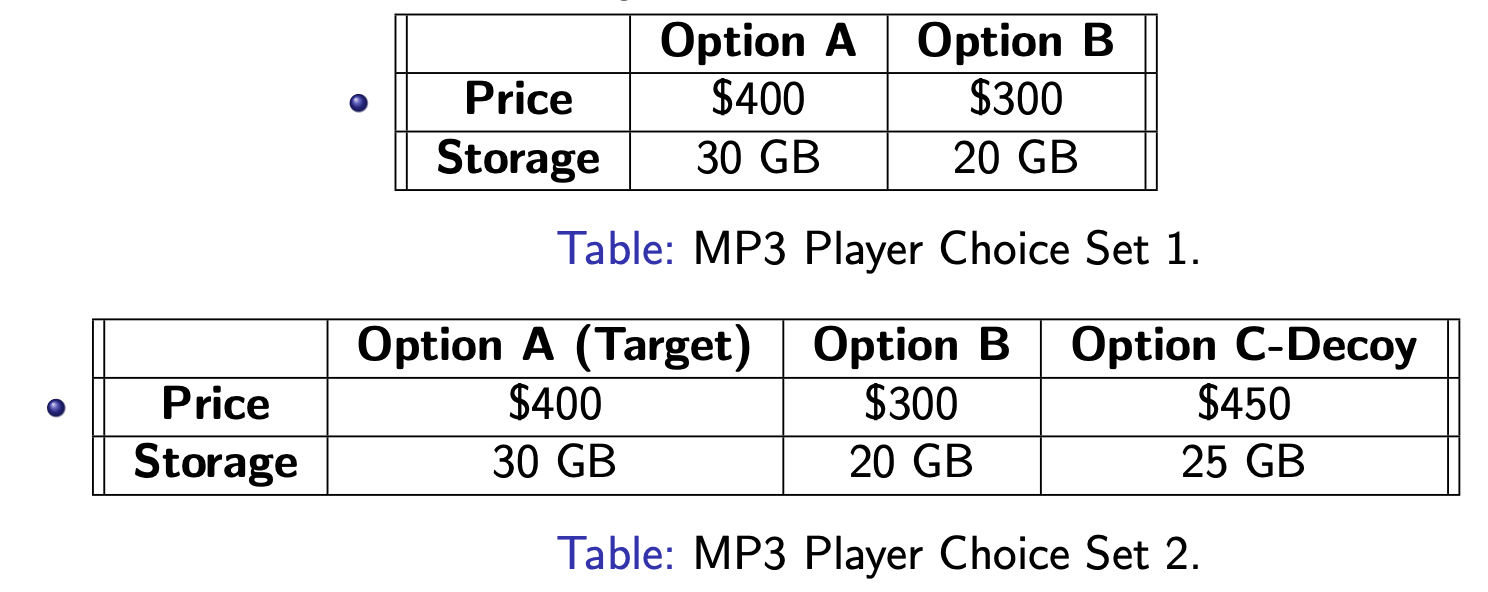
\includegraphics[scale=0.3]{CMNL1.png}
        \caption{Attraction Effect-Decoy Effect}
        \label{}
    \end{figure}\end{center}
    \item \textbf{The compromise Effect:} Middle option gets more share. In particular, in presence of this effect, when adding an extreme option (very high-level or basic product), the share of the middle-level options will increase.
    
    For example, a car-shopper who is given three options:
    \begin{enumerate}[1.]
        \item the low-priced basic model with no extras,
        \item a high-priced fully loaded model with all the extras,
        \item and a mid-priced model with some extras,
    \end{enumerate}
    will most likely choose the middle option.
    \item \textbf{The Similarity Effect:} Adding an item will hurt the market share and perceived preference of the options which are similar to it more than the dissimilar options.
\end{enumerate}
\begin{center}\begin{figure}[htbp]
    \centering
    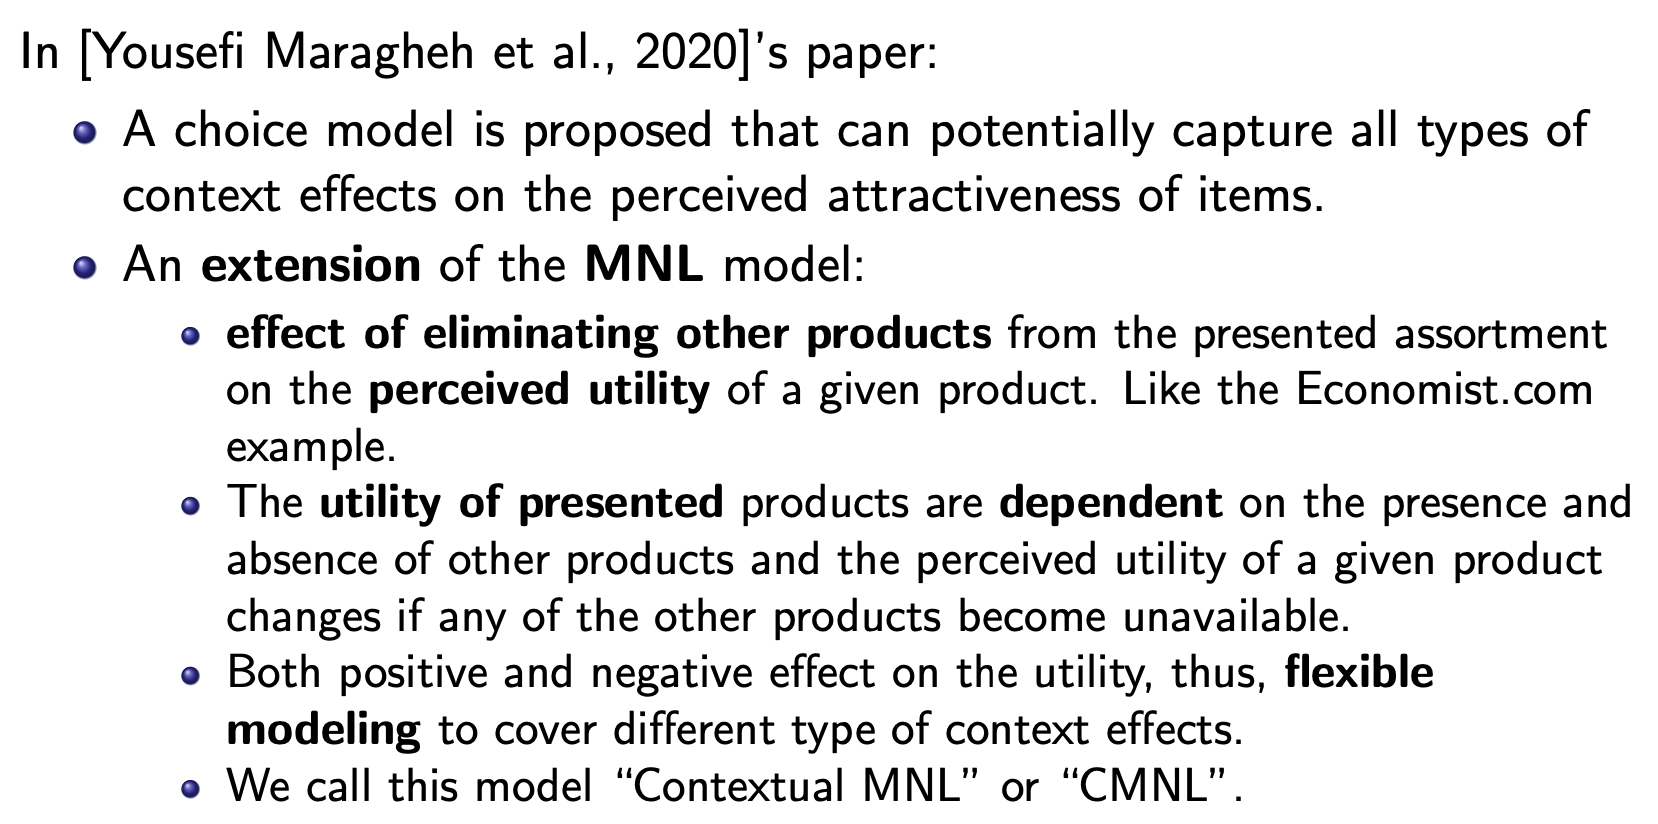
\includegraphics[scale=0.5]{CMNL2.png}
    \caption{CMNL}
    \label{}
\end{figure}\end{center}

\subsection{ Rank List-based Choice Model}
\subsubsection{ Motivation}
\begin{enumerate}[$\bullet$]
    \item Using historical sales data to predict the revenues or sales from offering a particular assortment of products to consumers.
    \item Fitting the ”right” parametric choice model to data are prone to overfitting and underfitting.
    \item The risk of model misspecification and leading to inaccuracies in decision making.
    \item Parametric models are prone to overfitting and underfitting.
    \begin{enumerate}
        \item Too simple model may make practically unreasonable assumptions.
        \item Too complex model can lead to worse performance.
    \end{enumerate}
    \item Need to make a data-driven, nonparametric choice model.
\end{enumerate}

\subsubsection{ Notations}
\begin{center}\begin{figure}[htbp]
    \centering
    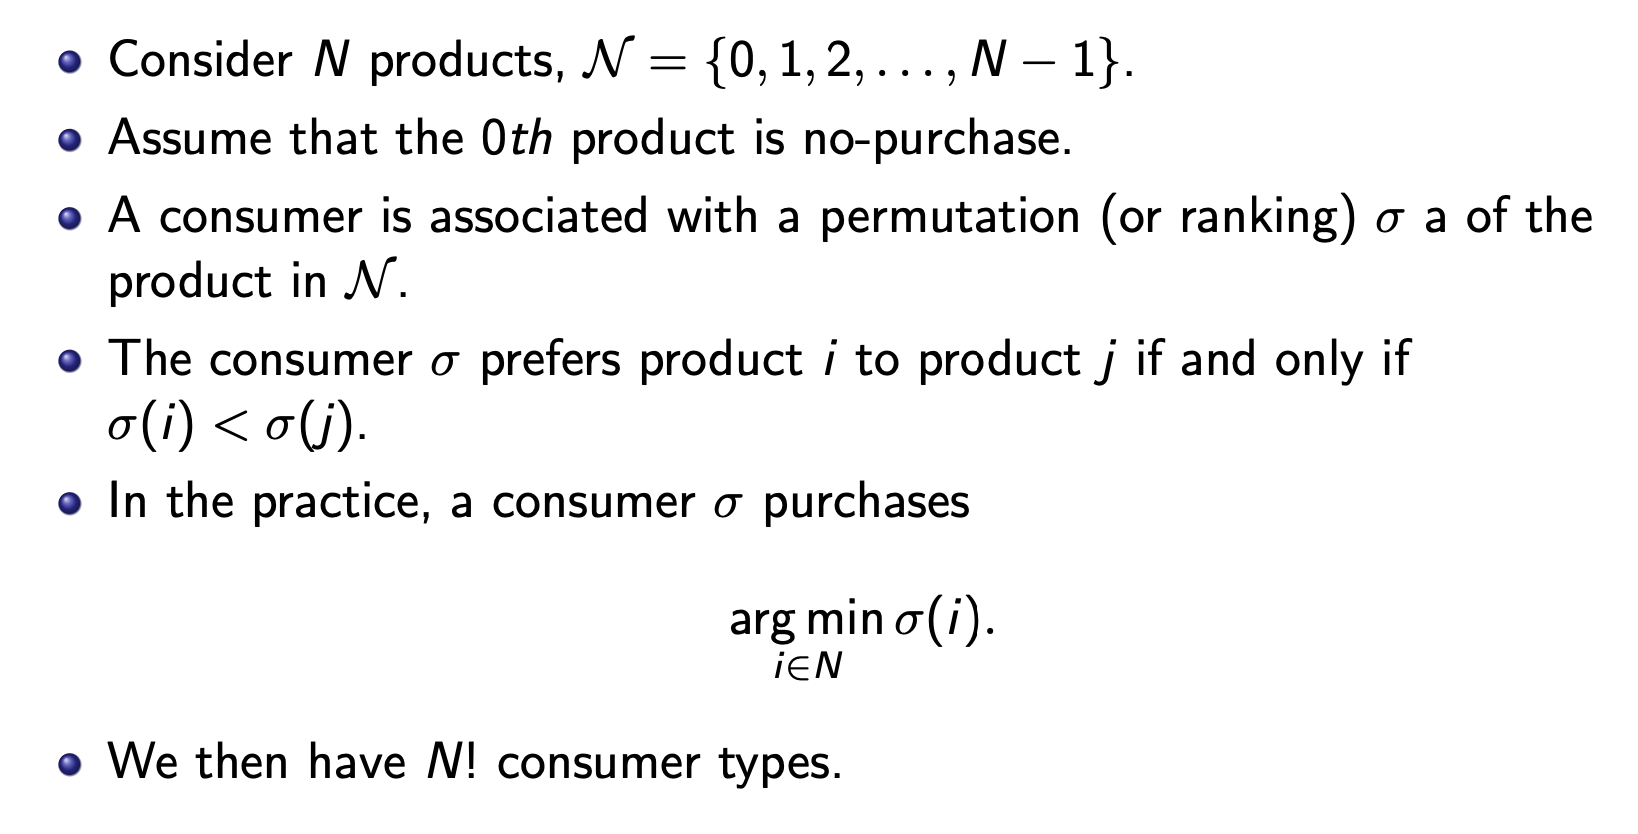
\includegraphics[scale=0.5]{RLCM1.png}
    \caption{Notations}
    \label{}
\end{figure}\end{center}

\subsubsection{ Model}
\begin{center}\begin{figure}[htbp]
    \centering
    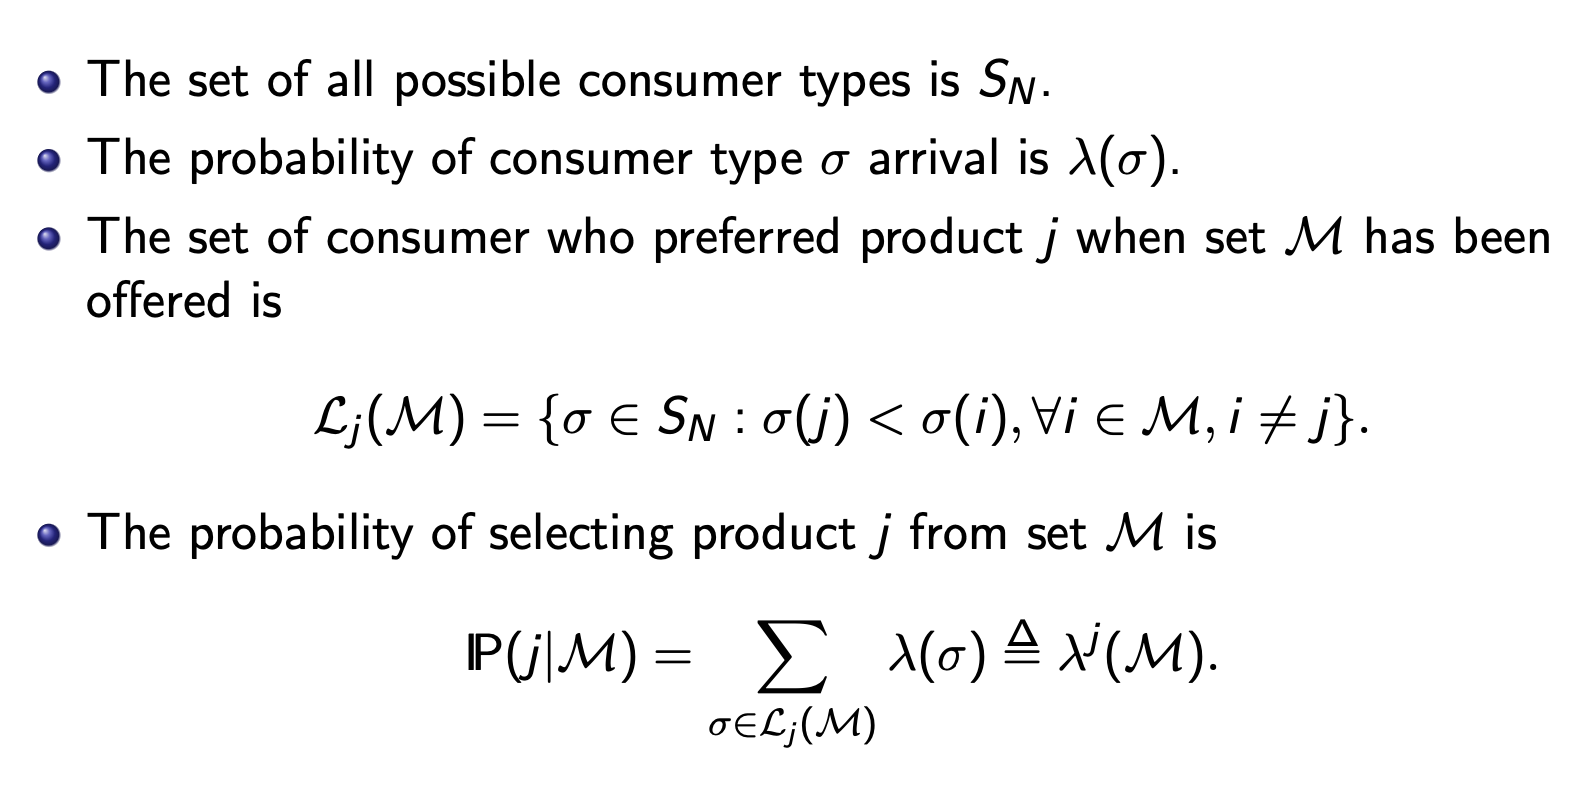
\includegraphics[scale=0.5]{RLCM2.png}
    \caption{Model}
    \label{}
\end{figure}\end{center}
\begin{center}\begin{figure}[htbp]
    \centering
    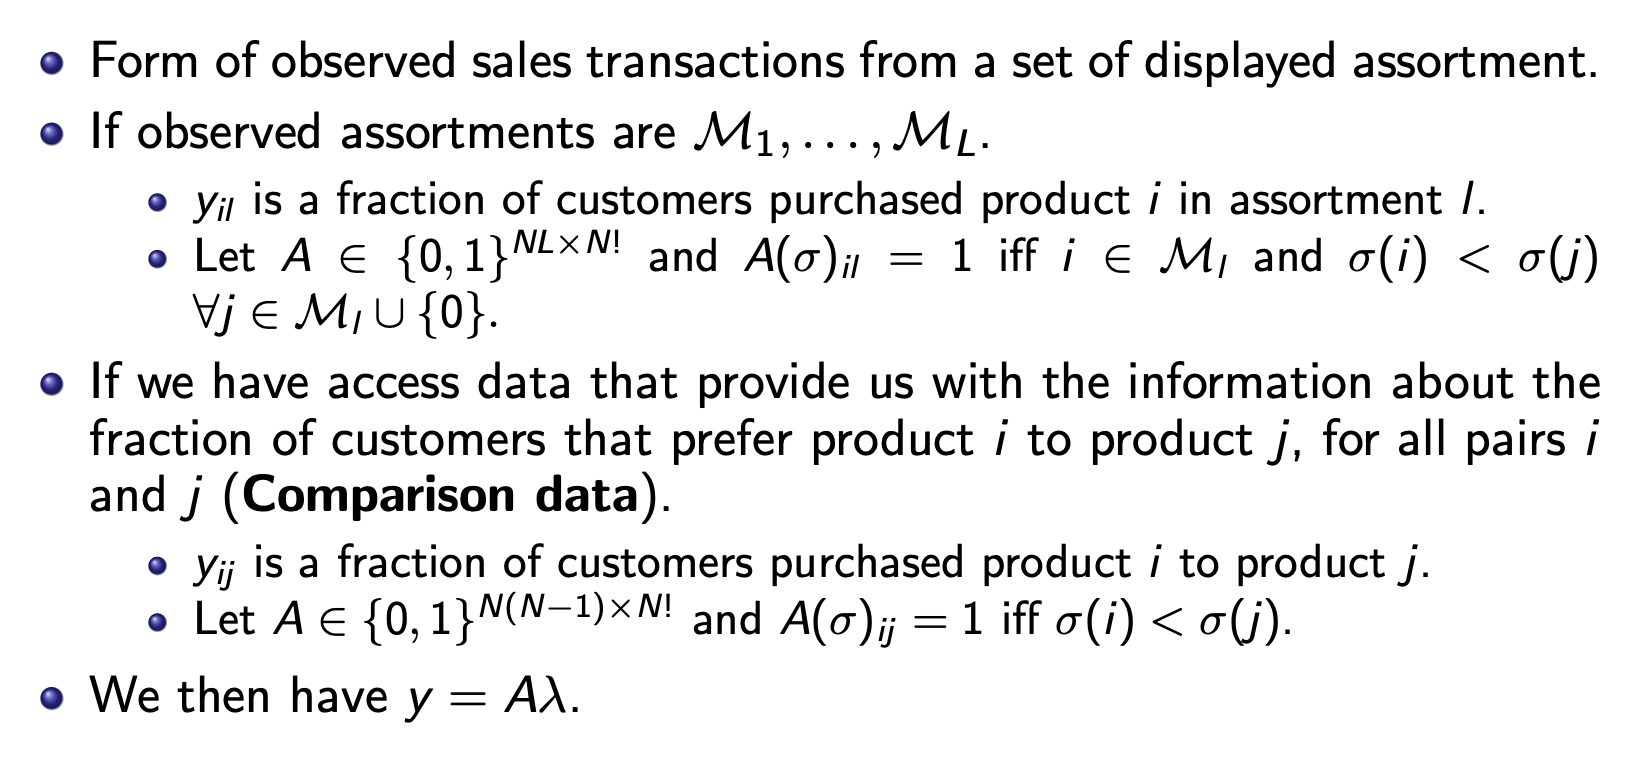
\includegraphics[scale=0.5]{RLCM3.png}
    \caption{Data}
    \label{}
\end{figure}\end{center}
\begin{center}\begin{figure}[htbp]
    \centering
    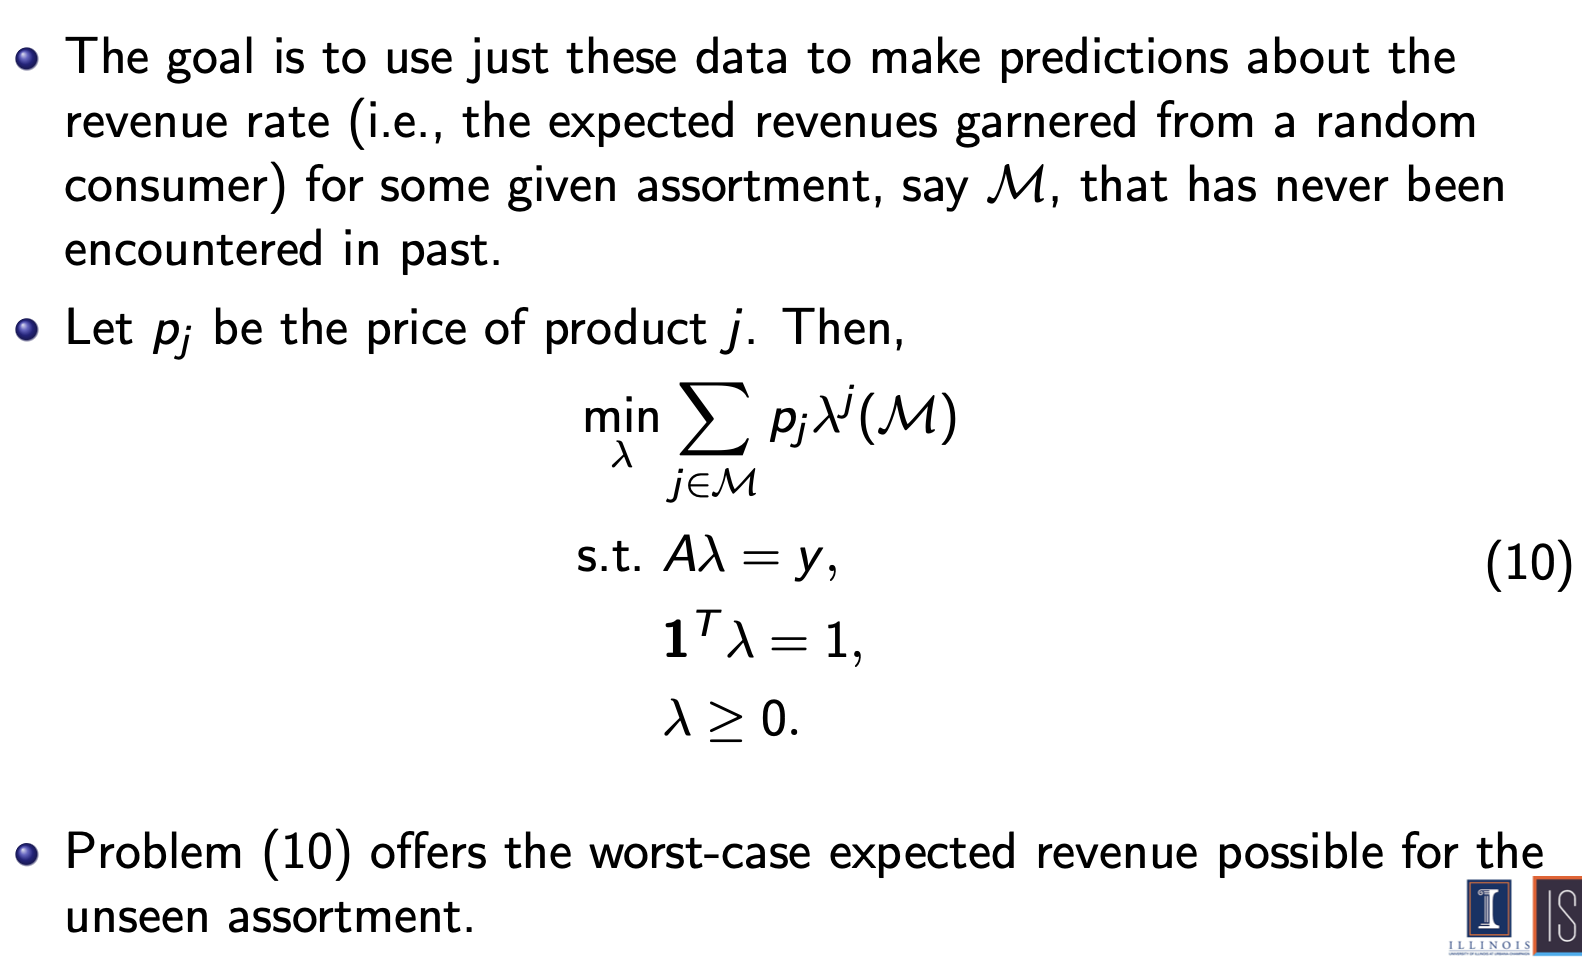
\includegraphics[scale=0.5]{RLCM4.png}
    \caption{Robust Approach}
    \label{}
\end{figure}\end{center}

\subsubsection{ Testing the Performance of Robust Approach}
\begin{center}\begin{figure}[htbp]
    \centering
    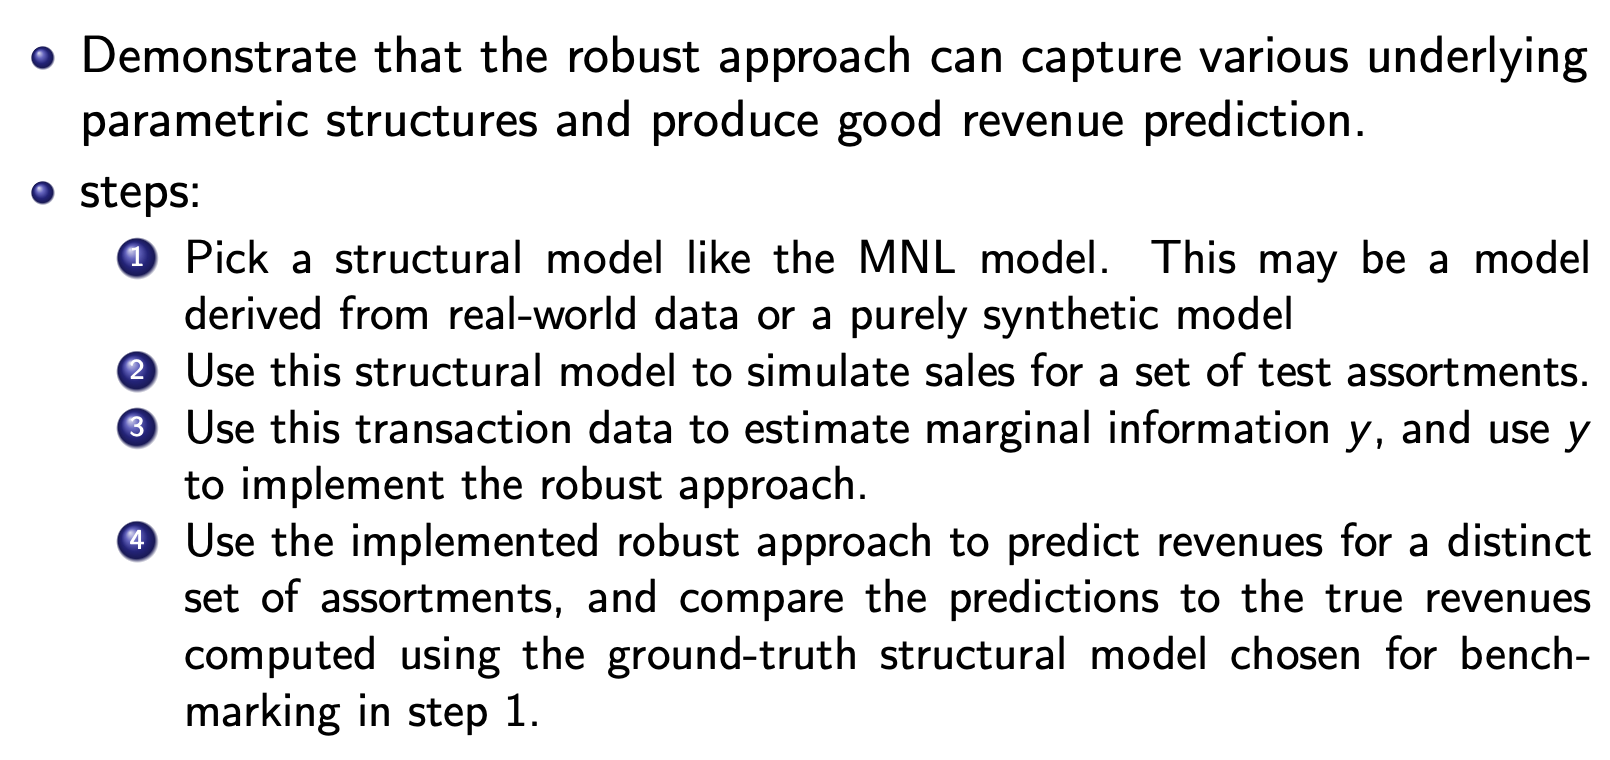
\includegraphics[scale=0.5]{RLCM5.png}
    \caption{Testing the Performance of Robust Approach}
    \label{}
\end{figure}\end{center}
\begin{center}\begin{figure}[htbp]
    \centering
    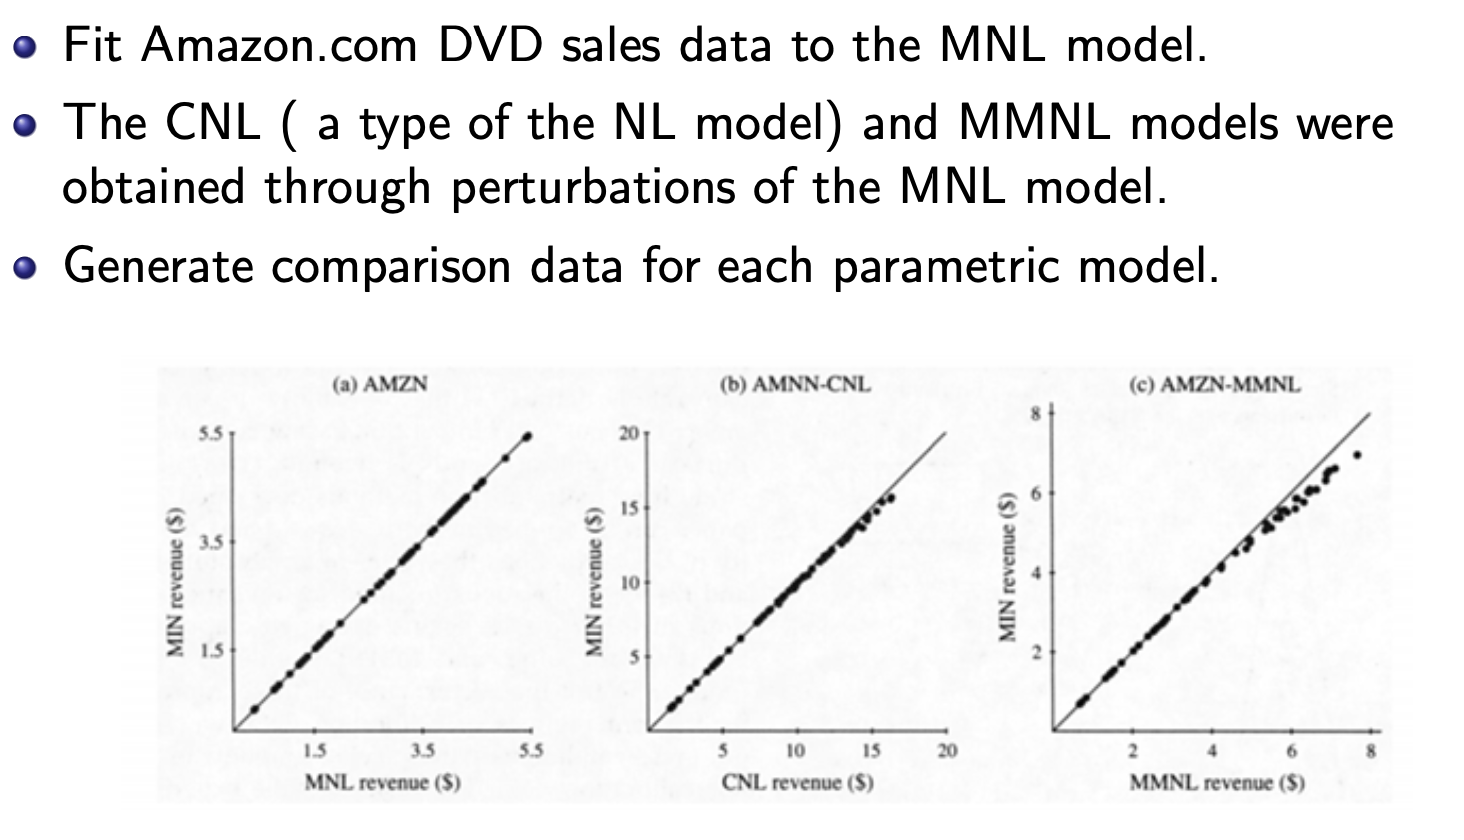
\includegraphics[scale=0.5]{RLCM6.png}
    \caption{Computational Study}
    \label{}
\end{figure}\end{center}

\subsubsection{ Limitations}
\begin{center}\begin{figure}[htbp]
    \centering
    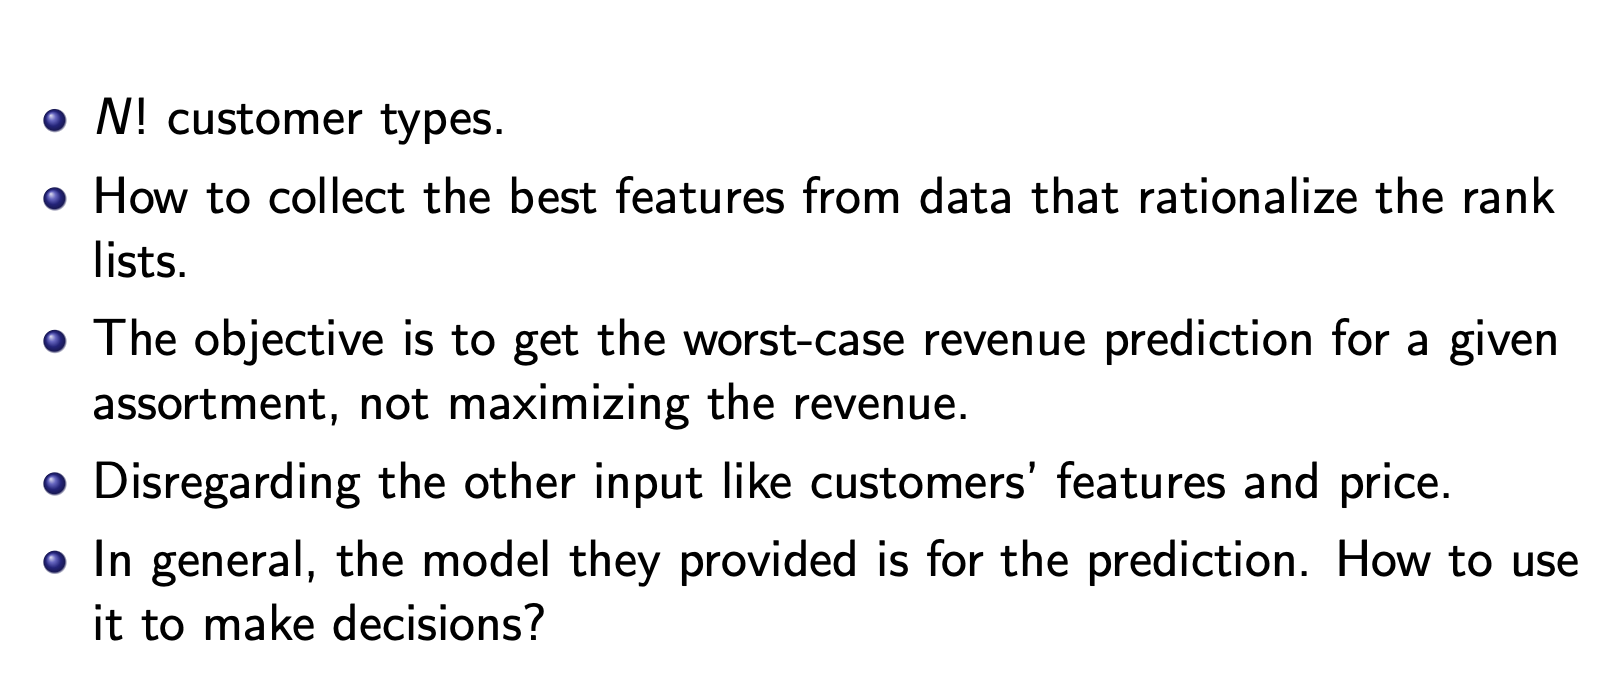
\includegraphics[scale=0.5]{RLCM7.png}
    \caption{Limitations}
    \label{}
\end{figure}\end{center}

\subsection{ Threshold Utility Model}
buy multiple products








\end{document}